

\documentclass[draft,grl]{agutexSI2019}


%
 \usepackage{graphicx}
 \usepackage{float}
%
%  Uncomment the following command to allow illustrations to print
%   when using Draft:
 \setkeys{Gin}{draft=false}

%% ------------------------------------------------------------------------ %%
%
%  ENTER PREAMBLE
%
%% ------------------------------------------------------------------------ %%

% Author names in capital letters:
\authorrunninghead{HOFER ET AL.}

% Shorter version of title entered in capital letters:
\titlerunninghead{Drifting snow and clouds Antarctica}

%Corresponding author mailing address and e-mail address:
\authoraddr{Corresponding author: Stefan Hofer,
(stefan.hofer@geo.uio.no)}

\begin{document}

%% ------------------------------------------------------------------------ %%
%
%  TITLE
%
%% ------------------------------------------------------------------------ %%

%\includegraphics{agu_pubart-white_reduced.eps}


\title{Supporting Information for "The contribution of drifting snow to cloud properties and the atmospheric radiative budget over Antarctica"}
%
% e.g., \title{Supporting Information for "Terrestrial ring current:
% Origin, formation, and decay $\alpha\beta\Gamma\Delta$"}
%
%DOI: 10.1002/%insert paper number here%

%% ------------------------------------------------------------------------ %%
%
%  AUTHORS AND AFFILIATIONS
%
%% ------------------------------------------------------------------------ %%


% List authors by first name or initial followed by last name and
% separated by commas. Use \affil{} to number affiliations, and
% \thanks{} for author notes.
% Additional author notes should be indicated with \thanks{} (for
% example, for current addresses).

% Example: \authors{A. B. Author\affil{1}\thanks{Current address, Antartica}, B. C. Author\affil{2,3}, and D. E.
% Author\affil{3,4}\thanks{Also funded by Monsanto.}}

\authors{Stefan Hofer\affil{1}, Charles Amory\affil{2,3}, Christoph Kittel\affil{2}, Tim Carlsen\affil{1},\\ Louis Le Toumelin\affil{4}\,and Trude Storelvmo\affil{1}}

\affiliation{1}{Department of Geosciences, University of Oslo, Oslo, Norway}
\affiliation{2}{Laboratory of Climatology, SPHERES Research Unit, University of Liège, Liège, Belgium}
\affiliation{3}{Univ. Grenoble Alpes, CNRS, Institut des Géosciences de l’Environnement, Grenoble, France}
\affiliation{4}{Univ. Grenoble Alpes, Université de Toulouse, Météo-France, CNRS, CNRM, Centre d’Études de la Neige, Grenoble, France}

%(repeat as many times as is necessary)





%% ------------------------------------------------------------------------ %%
%
%  BEGIN ARTICLE
%
%% ------------------------------------------------------------------------ %%


\begin{article}



\noindent\textbf{Contents of this file}
%%%Remove or add items as needed%%%
\begin{enumerate}
\item Figure S1
\item Figure S2
\item Figure S3
\end{enumerate}


%Type or paste caption here.
%upload your audio file(s) to AGU's journal submission site and select "Supporting Information %(SI)" as the file type. Following naming convention: auds01.


%Repeat for any additional Supporting audio files

%%% End of body of article:
%%%%%%%%%%%%%%%%%%%%%%%%%%%%%%%%%%%%%%%%%%%%%%%%%%%%%%%%%%%%%%%%
%
% Optional Notation section goes here
%
% Notation -- End each entry with a period.
% \begin{notation}
% Term & definition.\\
% Second term & second definition.\\
% \end{notation}
%%%%%%%%%%%%%%%%%%%%%%%%%%%%%%%%%%%%%%%%%%%%%%%%%%%%%%%%%%%%%%%%


%% ------------------------------------------------------------------------ %%
%%  REFERENCE LIST AND TEXT CITATIONS

%%%%%%%%%%%%%%%%%%%%%%%%%%%%%%%%%%%%%%%%%%%%%%%
% 
%
%
% no need to specify bibliographystyle
%
% Note that ALL references in this supporting information file must also be referenced in the primary manuscript
%
%%%%%%%%%%%%%%%%%%%%%%%%%%%%%%%%%%%%%%%%%%%%%%%
% if you get an error about newblock being undefined, uncomment this line:
%\newcommand{\newblock}{}

% \bibliography{ uncomment this line and enter the name of your bibtex file here } 




%Reference citation instructions and examples:
%
% Please use ONLY \cite and \citeA for reference citations.
% \cite for parenthetical references
% ...as shown in recent studies (Simpson et al., 2019)
% \citeA for in-text citations
% ...Simpson et al (2019) have shown...
% DO NOT use other cite commands (e.g., \citet, \citep, \citeyear, \nocite, \citealp, etc.).
%
%
%...as shown by \citeA{jskilby}.
%...as shown by \citeA{lewin76}, \citeA{carson86}, \citeA{bartoldy02}, and \citeA{rinaldi03}.
%...has been shown \cite<e.g.,>{jskilbye}.
%...has been shown \cite{lewin76,carson86,bartoldy02,rinaldi03}.
%...has been shown \cite{lewin76,carson86,bartoldy02,rinaldi03}.
%
% apacite uses < > for prenotes, not [ ]
% DO NOT use other cite commands (e.g., \citet, \citep, \citeyear, \nocite, \citealp, etc.).
%

%% ------------------------------------------------------------------------ %%
%
%  END ARTICLE
%
%% ------------------------------------------------------------------------ %%
\end{article}
\clearpage
\begin{figure}[H]
	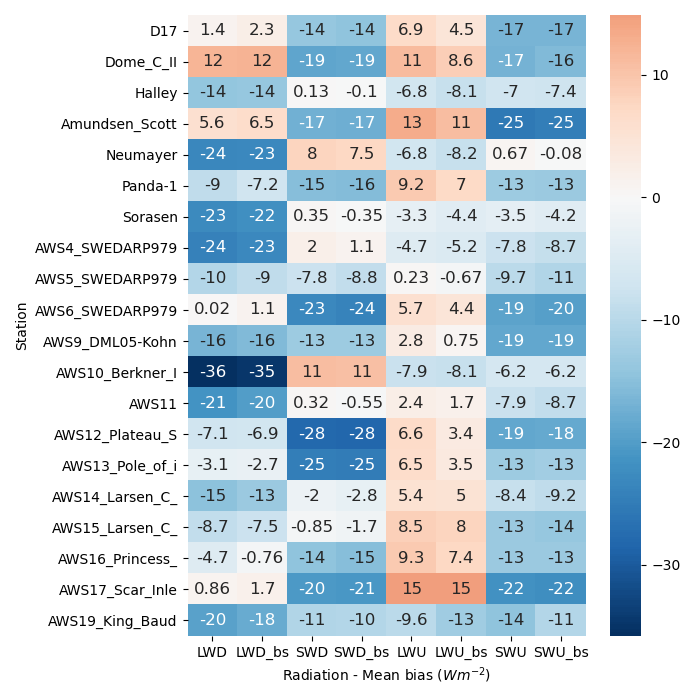
\includegraphics[width=0.9\textwidth]{heatmap_all_mb_new.png}
	\caption{\textbf{Complete statistical comparison of MAR to 20 in-situ weather stations over Antarctica.} Mean bias (Wm\textsuperscript{-2}) of the MAR simulations without drifting snow (e.g. "LWD") and MAR with drifting snow (e.g. "LWD\_bs") compared to 20 Antarctic-wide in-situ weather observations.}
	\label{fig:heat_all}
\end{figure}

\begin{figure}[H]
	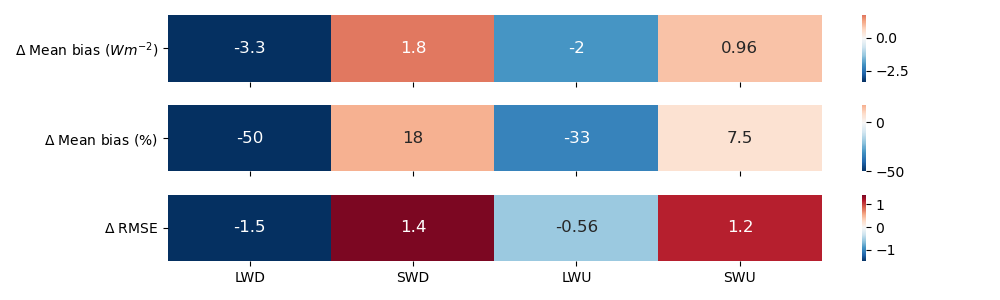
\includegraphics[width=0.9\textwidth]{heatmap_bs_days.png}
	\caption{\textbf{Statistical comparison of MAR to 20 in-situ weather stations over Antarctica during drifting snow days.} Mean bias (Wm\textsuperscript{-2}) of the MAR simulations without drifting snow (e.g. "LWD") and MAR with drifting snow (e.g. "LWD\_bs") compared to 20 Antarctic-wide in-situ weather observations during drifting snow days only. We defined drifting snow days as these days where the daily mean drifting snow exceeds a snow transport of 3.2$\cdot$10\textsuperscript{-3} kg$\cdot$m\textsuperscript{-2}, based on observations made at the two stations of Antarctica that observe blowing snow directly (D17 and D47, \cite{amory2021, Letoumelin2020}).}
	\label{fig:heat_bs}
\end{figure}

\begin{figure}[H]
	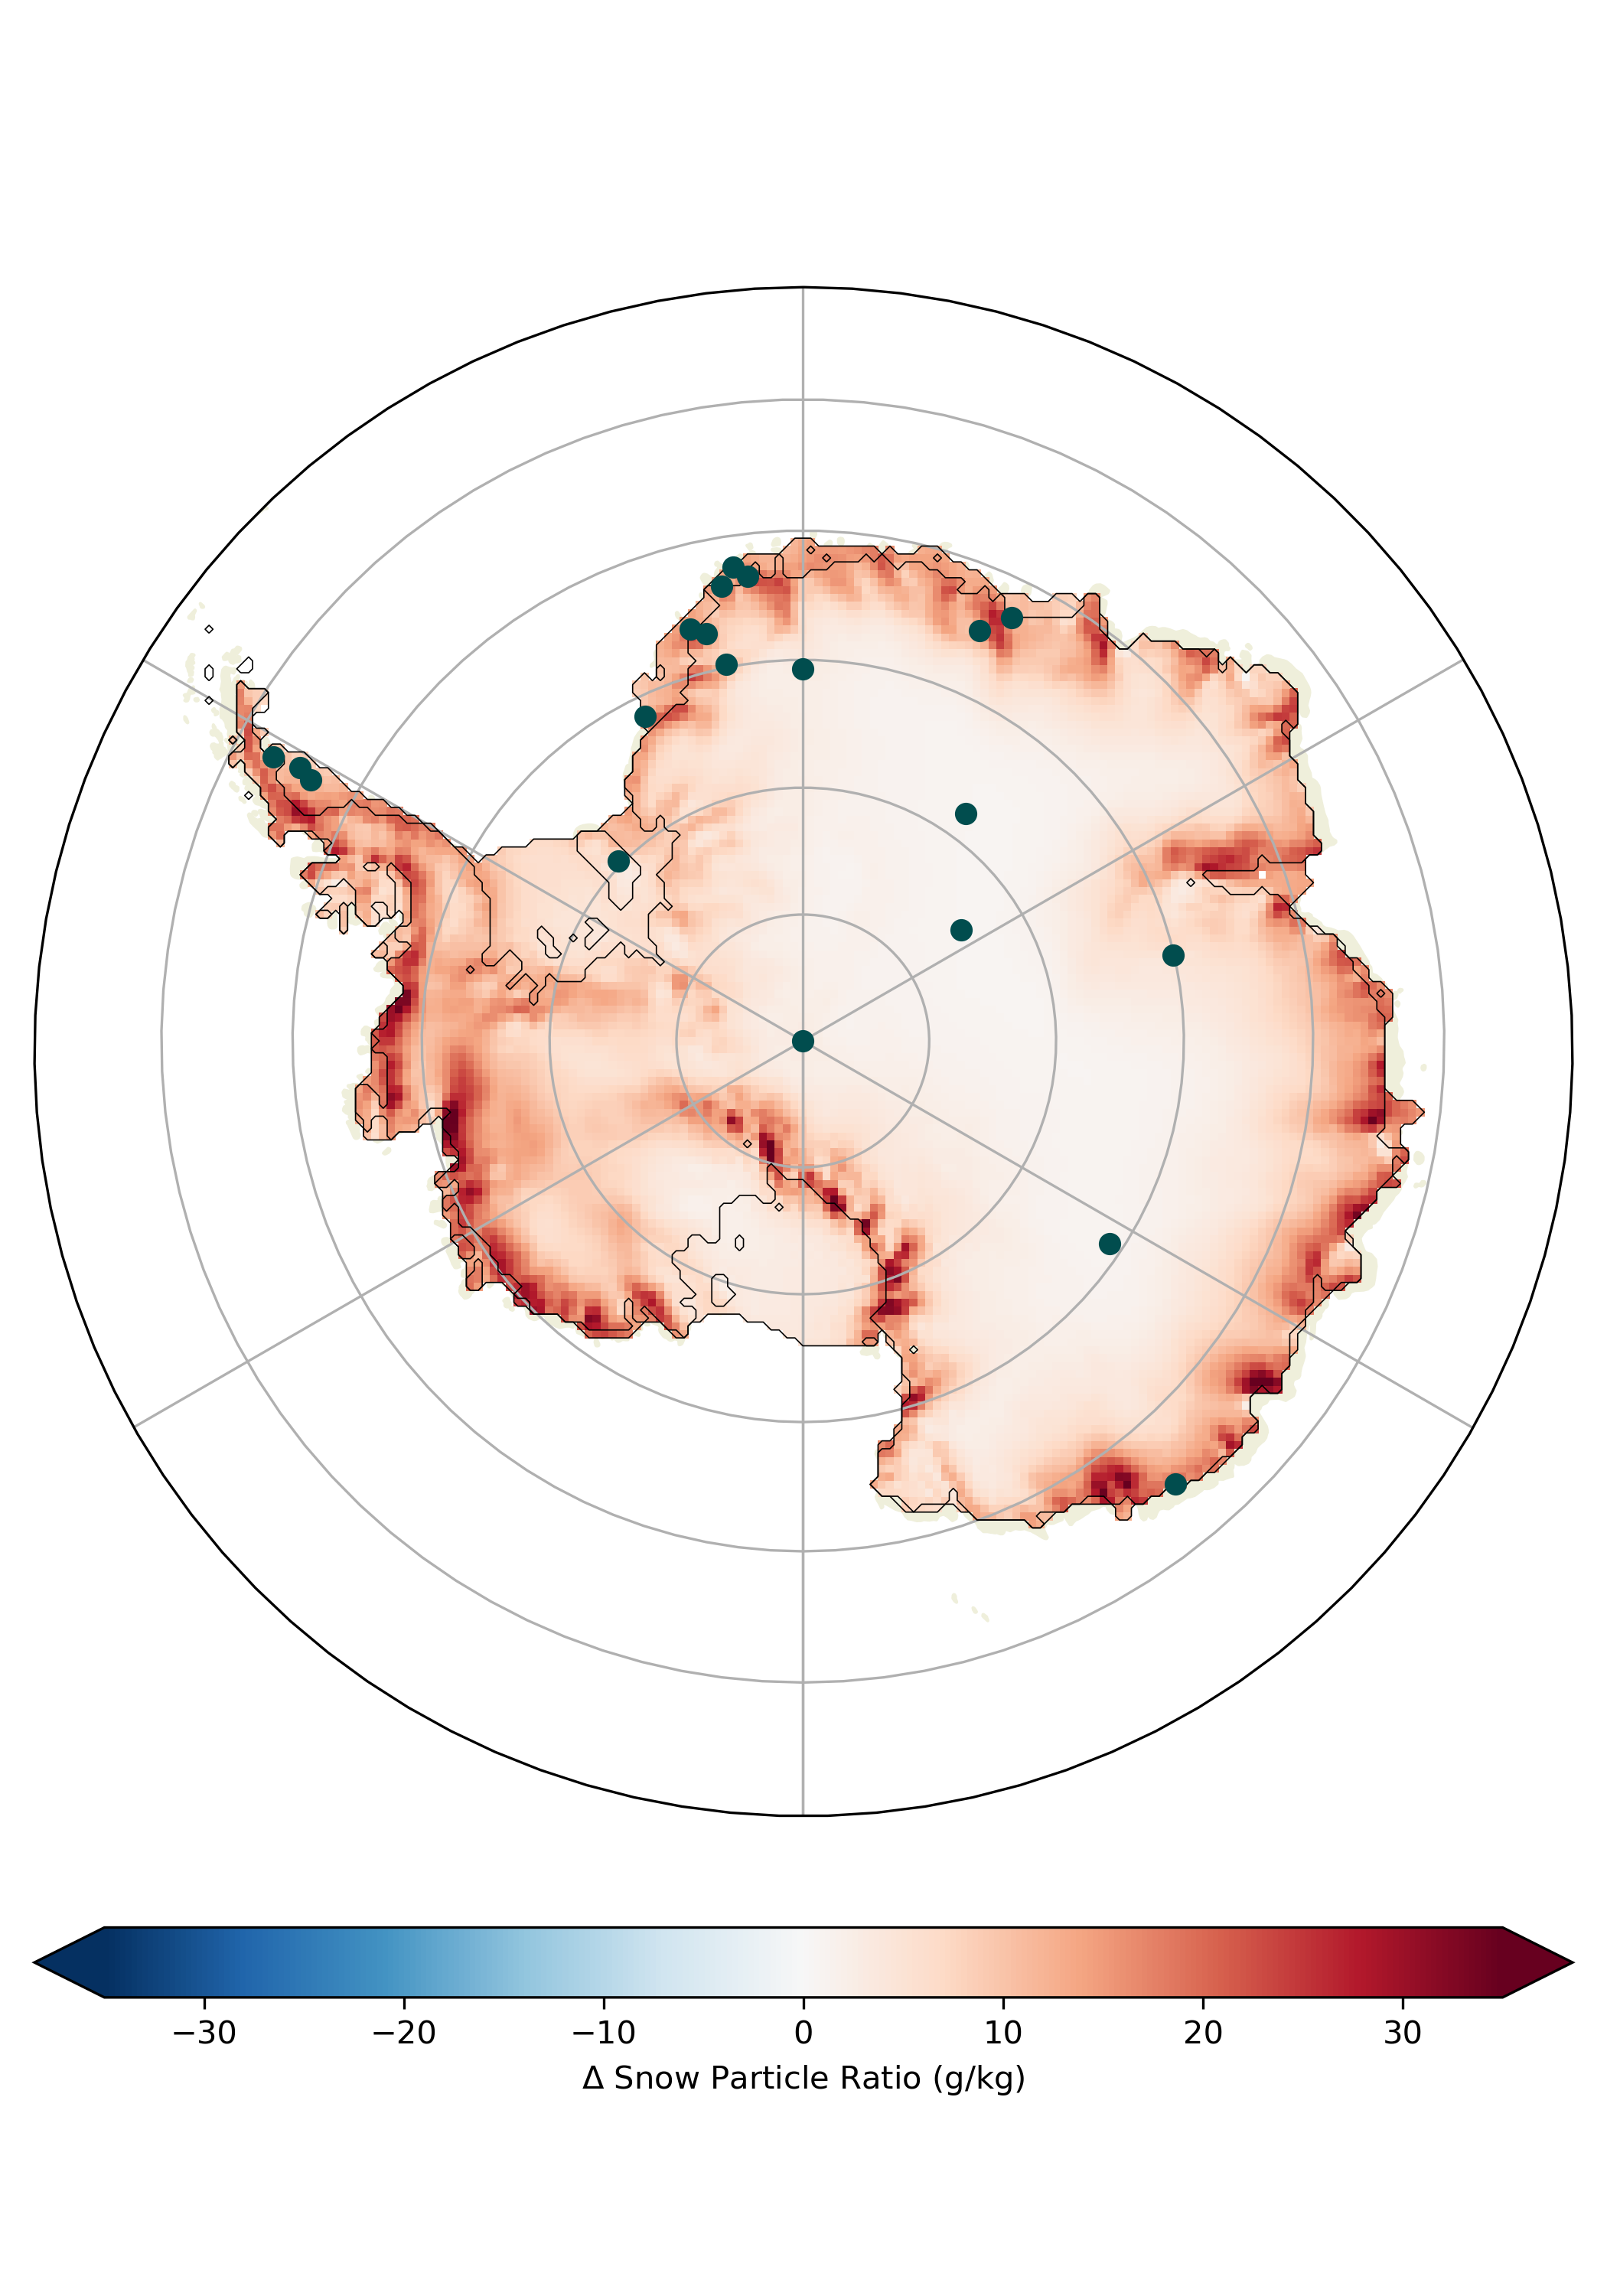
\includegraphics[width=0.7\textwidth]{station_map.png}
	\caption{\textbf{Location of the 20 automatic weather stations used in this study.} Overview of the geographic distribution of the 20 AWS station used in this study for the model validation. The background colors show the 2000-2019 average of the snow particle ratio (g/kg) from the MAR model.}
	\label{fig:stations}
\end{figure}

\bibliography{agusample}


\end{document}

